\chapter{Function calls with timeouts, revisited: \\ the \textit{libinger} library}
\label{chap:libinger}

\ifdefined\chapquotes
\vspace{-0.5in}
\begin{chapquote}[1.5in]{David Mitchell, \textit{Cloud Atlas}}
A half-read book is a half-finished love affair.
\end{chapquote}
\fi

In Chapter~\ref{chap:functions}, we introduced and motivated lightweight preemptible
functions, a novel concurrency abstraction pairing synchronous invocation with
preemption.  At that time, we covered the design principles underlying the API for
managing preemptible functions; in this chapter, we will discuss the API itself in
more detail and the design and implementation of \textit{libinger}, the library that
provides preemptible functions.

We start by giving the full \textit{libinger} C interface in
Listing~\ref{lst:ingerfullapi}.  The \texttt{launch()} and \texttt{resume()}
functions work as already described:\@ the former creates a new preemptible function
and lets it run on the caller's thread for the specified number of microseconds
(which may be zero), and the latter resumes a preemptible function that had become
paused after exhausting its time budget.  The new \texttt{cancel()} function allows
the caller to discontinue a paused preemptible function rather than allowing it to
run to completion.  Finally, the \texttt{pause()} function may be called from within
a preemptible function to cooperatively yield.  It immediately pauses the function
and returns to its caller, just as if the function had been preempted.

The Rust interface appears in Listing~\ref{lst:ingerrustapi} and differs in several
important ways:

\begin{figure}
\begin{lstlisting}[label=lst:ingerfullapi,caption=Preemptible functions extended C interface,morekeywords=uint64_t]
struct linger_t {
	bool is_complete;
	cont_t continuation;
};

typedef void (*Function)(void *);

linger_t launch(Function func,
                  uint64_t time_us,
                  void *args);
void resume(linger_t *cont, uint64_t time_us);
void cancel(linger_t *cont);
void pause(void);
\end{lstlisting}
\end{figure}

\begin{figure}
\begin{lstlisting}[label=lst:ingerrustapi,caption=Preemptible functions Rust interface,morekeywords={fn,impl,mut,pub,self,u64,Drop,FnOnce,Result,Send}]
pub enum Linger<T> {
	Completion(T),
	Continuation(Continuation),
	Poison,
}

pub fn launch<T: Send>(func: impl FnOnce() -> T + Send,
			 time_us: u64) -> Result<Linger<T>>;
pub fn resume<T>(func: &mut Linger<T>,
		   time_us: u64) -> Result<&mut Linger<T>>;
pub fn pause();

impl<T> Linger<T> {
	pub fn yielded(&self) -> bool;
}

impl Drop for Continuation { ... }
\end{lstlisting}
\end{figure}


\paragraph{Closure support.}
We leverage Rust's first-class closures to enable the caller to pass
\texttt{launch()} a function that captures state from its environment.  We expect the
caller to provide any inputs to the function in this manner.  Unlike with the C
interface, there is no need to wrap the arguments in a struct when there are
multiple, or to pass an empty value when there are none.


\paragraph{Type safety.}
The aforementioned interface change means that the Rust wrapper functions do not
erase the types of the preemptible function's parameters by diluting them to a
\texttt{void *}; thus, the preemptible function does not have to perform an unsafe
cast before using them, and the compiler can still type check the program.
Furthermore, both \texttt{launch()} and \texttt{resume()} are generic on the
preemptible function's return type:\@ instead of a \texttt{linger\_t}, they return a
tagged union.  Once the preemptible function runs to completion, the caller may
destructure this type to retrieve the function's return value.  Because the union is
tagged, it is impossible to destructure it to retrieve the return value unless the
function has truly run to completion.


\paragraph{RAII.}
Our Rust interface adheres to the RAII (Resource Allocation Is Initialization) idiom,
allowing continuation deallocation to happen automatically.  Unlike the C interface,
the Rust one has no \texttt{cancel()} function; instead, its continuation objects
implement the language's \texttt{Drop} trait.  Whenever a continuation goes out of
scope without being consumed by running to completion, the language calls its
destructor, which implicitly performs a cancellation.


\paragraph{Safe concurrency.}
The \texttt{launch()} function requires that the preemptible function closure
implement the language's \texttt{Send} trait, which is true provided that all of the
values it captures have this trait.  In Rust, a type is \texttt{Send} if and only if
ownership of it can be safely transferred between threads.  This includes all objects
that do not contain any references, as well as those that do but only to data that is
safe to access concurrently (\texttt{Sync} in Rust parlance)~\cite{www-rustlang-conc}.
This restriction on
the closure means that any attempt to share state between a caller and its
preemptible function without the use of appropriate concurrency control will fail at
compile time.


\paragraph{Flexibility.}
The requirement that Rust preemptible functions be \texttt{Send} is similar to the
restrictions imposed by the standard library's thread \texttt{spawn()} interface.
However, \texttt{launch()} differs in an important way:\@ unlike a thread, a
preemptible function is not restricted to the \texttt{'static} lifetime, and so is
able to accept references to local variables and other dynamically-allocated data.
In contrast, attempts to transfer such references to a thread would result in a
compile error.  What makes it safe to use all lifetimes with preemptible functions is
the fact that they execute synchronously, and therefore cannot outlive the calling
context without first becoming paused.  If a preemptible function times out, the Rust
compiler knows the lifetime of any references it has captured, so any attempt to pass
the paused closure to a scope where its shared data no longer exists will be met with
a compile error.


\paragraph{Composability.}
In addition to the closure being \texttt{Send}, the opaque \texttt{Continuation} type
is as well.  This means that a preemptible function can be launched on one thread,
become paused, then be moved to another thread and resumed there.  Applications may
use this trick to move long-running tasks off the critical path, but it is especially
important for implementing thread libraries.  In fact, as we will see in
Chapter~\ref{chap:libturquoise}, it makes it easy to implement preemptive thread
libraries in userland.


\section{Shared responsibility for concurrency control}

The preceding points about concurrency restrictions in the Rust API may seem
incongruous with Chapter~\ref{chap:libgotcha}, which spent dozens of pages
introducing selective relinking, a technique billed as solving the concurrency perils
of preemptible functions.  In fact, that runtime exists to address a completely
separate (but equally critical) problem.

Adding preemptible functions to an application actually introduces two distinct forms
of concurrency.  Both stem from the fact that code within the same thread is now
allowed to interleave its execution at almost entirely arbitrary points, but they
differ in whether the code in question can possibly anticipate this problem, and
therefore have any hope of addressing it.

First, there is concurrency involving the libraries that the program depends on, many
of which were probably authored by third parties.  Although such libraries now
execute concurrently with preemptible functions by virtue of being used from the same
kernel thread, they conceptually ``predate'' preemptible functions' existence; that
is, they cannot even be expected to be aware of this concurrency.  The job of
\textit{libgotcha} is to reconcile this, first by establishing an isolation boundary
between each library (and the executable, for that matter) and the rest of the
program, and then by deferring preemption where shared state is still unavoidable.

Separately, there is concurrency involving the code that uses the preemptible
functions abstraction (i.e., implements and invokes preemptible functions).  Not only
\textit{can} this code take measures to ensure this concurrency is safe:\@ it has to
be the one to do so.  This is because there is often a legitimate need to explicitly
exchange information between a preemptible function and the surrounding program, in
which case the possibility of interleaving must be directly confronted.  As a simple
example, consider a preemptible function that is populating some data structure for
later use by the rest of the program.  Imagine that the function exhausts its
time budget and the application is running behind schedule and opts to cancel it.
Should the application need to retrieve the work done so far, it must use its
knowledge of how the preemptible function mutates the data structure to individually
validate each portion thereof before trusting it to be in a consistent state.  (The
preemptible function can make this easier by exposing a record of its progress that
indicates what parts of its data structures are consistent.)

Even without using cancellation, the traditional hazards of concurrency arise, just
as they do with state-of-the-art abstractions.  This problem space has long posed a
challenge to systems programmers, and we do not pursue any novel solution.  When
using the C interface, the programmer bears complete responsibility for writing code
that is free of data races.  Our Rust API, however, leverages that language's
first-class concurrency support so the compiler can catch such mistakes.


\subsection{Locking and deadlocks}
\label{sec:libinger:locks}

While the Rust compiler rejects all code that shares state unsafely, it is still
possible to introduce correctness bugs such as deadlock~\cite{www-rustlang-nu}.  This
is nothing new, a common cause being an ordinary function blocking on a
mutual-exclusion lock that is already held by its caller.  But it is especially easy
to make this mistake with preemptible functions.  The developer must remember that
each preemptible function runs on the same thread as its caller, so blocking is not a
legitimate way for a preemptible function to synchronize except with independent
threads.

Still, it is sometimes necessary for a preemptible function to protect a non-atomic
resource from other code on the same thread.  This is possible to do with yielding.
When a preemptible function needs to acquire a mutex, it should use a try lock
operation instead of a blocking lock.  If it fails to acquire exclusive access, it
should call \texttt{pause()} and wait for the caller to reschedule it at a later time
when the resource is hopefully available.  To make this more ergonomic, one could
easily build a custom mutex type that used this algorithm to implement its ``blocking
lock'' operation when called from a preemptible function.

The Rust API includes a \texttt{yielded()} method that the caller can use to
determine whether a preemptible function paused cooperatively.  This can be used to
implement the equivalent of deadlock detection for situations where multiple
preemptible functions are contending for a resource.


\section{Launching a preemptible function}

Invoking the \texttt{launch()} wrapper function with a nonzero time limit does the
following:
\begin{enumerate}
\item Allocates and installs a private thread control block specific to the preemptible function (Section~\ref{sec:libinger:tcbs})
\item Captures a snapshot of the kernel thread's execution context (Section~\ref{sec:libinger:contexts})
\item Allocates and switches to a private execution stack specific to the preemptible function (Section~\ref{sec:libinger:stacks})
\item Allocates a preemption signal specific to the kernel thread (Section~\ref{sec:libinger:signals})
\item Records a timestamp shortly before invoking the preemptible function (Section~\ref{sec:libinger:pausing})
\item Allocates and switches to a private libset specific to the preemptible function (Section~\ref{sec:libinger:isolation})
\item Invokes the preemptible function (Section~\ref{sec:libinger:jumps})
\end{enumerate}

Several of these steps involve allocating resources assigned to each preemptible
function.  Some of these allocations are slow as currently implemented, but the
resources are reusable once a preemptible function has completed or been cancelled.
We use pool allocators to automatically reuse released resources when available.  To
take expensive operations off the critical path, some of the allocators preallocate a
number of instances up front.

The following sections discuss each of the preemptible function invocation steps in
detail.


\section{Thread control blocks}
\label{sec:libinger:tcbs}

As discussed in Section~\ref{sec:libgotcha:tls}, \textit{libgotcha} leaves it to
control libraries to decide the scope of thread-local variables.  However, the
preemptible functions Rust API constrains \textit{libinger}'s choice in the matter.
Because the \texttt{Continuation} type is \texttt{Send}, preemptible functions may
resume execution on a different thread than they were running on before becoming
paused.  To prevent their thread-local variables from changing out from under them,
we therefore associate thread-local variables with the preemptible function instead
of the thread.  Application programmers should be aware that, unlike global
variables, thread locals' values are not shared between a preemptible function and
its defining module.\footnote{Users of thread pools built on top of preemptible
functions need not be aware of this detail, or even of preemptible functions.  This
is because thread pool users must already assume their task will be scheduled on a
different thread than the code that submitted it.}

To allocate a thread control block, \textit{libinger} calls the dynamic linker's
\texttt{\_dl\_allocate\_tls()} function (the same one used by
\texttt{pthread\_create()}).  This function creates a TCB and accompanying TLS area,
but only initializes the latter.  Unfortunately, there are a few TCB fields that must
be initialized for the thread to operate properly, so \textit{libinger} manually sets
those.\footnote{Two of these are self-referential pointers back to the beginning of
the TCB: one is for finding the TLS area (which is located just before the
TCB), and one is the thread identifier returned by \texttt{pthread\_self()}.  There
is also a pointer guard field that glibc uses to decode some of its internal pointers
that are mangled as an exploit mitigation, and a field containing the kernel's thread
identifier.}  It then calls \texttt{\_\_ctype\_init()} to select the correct
\texttt{ctype.h} implementations for the locale.  Thread control blocks are one of
the resources it pool allocates and reuses unless a preemptible function is
cancelled.  This choice was informed by the expense of allocating TCBs as seen in
Section~\ref{sec:libgotcha:libtlsblock}; however, it is possible to instead reduce
this cost using a technique like the one we prototyped in that section.

To install the TCB, we need to load it into the thread segment register using
\texttt{arch\_prctl()}.  This is one of the functions that \textit{libgotcha}
wraps (Section~\ref{sec:libgotcha:interpose}); since \textit{libinger} is an internal
control library, it calls \texttt{libgotcha\_arch\_prctl()} instead to also notify
\textit{libgotcha} of the change.


\section{Execution contexts}
\label{sec:libinger:contexts}

The \texttt{Continuation} type inside a paused preemptible function must contain
enough information to resume the function's execution from where it left off, which
could be any program point because we interrupt asynchronously.  To capture a
snapshot
of the machine registers, we use POSIX contexts, a mechanism for non-local jumps.
Unlike the better known \texttt{setjmp()}/\texttt{longjmp()} interface from the C
standard, POSIX contexts permit capturing an execution snapshot on one thread and
resuming it on another.

One of \texttt{launch()}'s early actions is to snapshot its own execution context.
It keeps this snapshot available while the preemptible function is running; if the
function times out, \textit{libinger} will use the snapshot to jump directly back
into \texttt{launch()} (or \texttt{resume()}), which will populate the
\texttt{Continuation} type and return it to the caller.


\subsection{Using POSIX contexts safely}
\label{sec:libinger:boilerplate}

Any nontrivial use of the POSIX contexts interface requires some surprisingly-subtle
boilerplate code.  Like the \texttt{setjmp()} function, the
\texttt{getcontext()} function can return multiple times:\@ it always returns once
when the snapshot is initially captured, but each subsequent restoration of the
context causes it to return again.  Unfortunately, it provides no indication of
whether it is returning for the first time, even though the caller almost always
needs to know.  For instance, we only want to launch the preemptible function after
we capture the snapshot, not after it is restored (in which case we want to package
the \texttt{Continuation} and return).  A simple boolean flag does not work because
the compiler is likely to store it in a register, so any updates after the capture
will be undone by the restore.  At a minimum, one must store the flag in a volatile
variable~\cite{getcontext-manpage}.

In C, getting the flag right would be enough boilerplate to use the context, as long
as we did so sensibly.  However, RAII in languages such as Rust makes it very easy to
implicitly create memory corruption.  Consider the example in
Listing~\ref{lst:ingerdoublefree}, which is correct as written but deceivingly
brittle.  It prints:
\begin{lstlisting}[language=]
  Snapshot was captured!
  About to restore snapshot!
  Snapshot was restored!
  Deallocating `closure`, `capturing`, and `snapshot`!
\end{lstlisting}

\begin{figure}
\begin{lstlisting}[label=lst:ingerdoublefree,caption=Subtly unsound use of POSIX contexts from Rust,morekeywords={let,mut,unsafe}]
unsafe {
	// Closure that runs once right after we capture the snapshot
	let closure = |snapshot| {
		println!("About to restore snapshot!");
		setcontext(snapshot);
	};

	// Flag to track whether we are capturing or restoring the snapshot
	let mut capturing = Volatile::from(true);

	// Checkpoint in the program
	let mut snapshot = MaybeUninit::uninit();
	getcontext(snapshot.as_mut_ptr());

	if capturing.read() {
		println!("Snapshot was captured!");
		capturing.write(false);
		closure(snapshot.assume_init_ref());
	} else {
		println!("Snapshot was restored!");
	}

	println!("Deallocating `closure`, `capturing`, and `snapshot`!");
}
\end{lstlisting}
\end{figure}

The closure here is of type \texttt{Fn(\&ucontext\_t) -> ()}, which means it takes a
reference to a POSIX context and returns nothing.  However, changing the code in the
closure might affect that type.  For example, imagine we had a type
\texttt{OneTimePadded} for storing data that could only be unwrapped once.  We might
want \texttt{closure} to capture such a value and ``decode'' it:
\begin{lstlisting}
  let secret = OneTimePadded::from("About to restore snapshot!");
  let closure = move |snapshot| {
  	println!("{}", secret.into_inner());
	setcontext(snapshot);
  };
\end{lstlisting}

If we make this substitution, the code still compiles.  The program's output
describes when the existing variables go out of scope, but how about the new
\texttt{secret} variable?  Recall that it can only be unwrapped once; therefore the
\texttt{secret.into\_inner()} call consumes it (by taking ownership).  When that call
returns, it will go out of scope and its destructor will be invoked.  This should be
troubling:\@ we said earlier that \texttt{closure} was in scope until the end of the
\texttt{unsafe} block, so it would seem that \texttt{closure} would have to live that
long as well (so that \texttt{secret} would still be deallocated if \texttt{closure}
were never called).

In fact, the Rust compiler is aware that the closure ``uses up'' its captured
variable.  The most important implication of this is that the closure can never be
called more than once, so the compiler has changed its type to
\texttt{FnOnce(\&ucontext\_t) -> ()}.  As with our imagined \texttt{into\_inner()}
method, calling a \texttt{FnOnce} closure consumes the closure.  For this reason, the
scope of \texttt{closure} has changed and it now gets deallocated either when it is
called or at the end of the \texttt{unsafe} block, depending on which branch is
taken.  Unfortunately, when we restore the snapshot, Rust does not know that the
\texttt{if} has already been taken, so it assumes it is in the latter situation and
deallocates \texttt{closure} at the end, calling \texttt{secret}'s destructor in the
process.  If \texttt{secret} includes any heap-allocated memory, this is a double
free.  Note that this unsoundness was introduced not because \texttt{closure} now
captures a variable, but because it \textit{consumes} that variable.

Programmers might need to write preemptible functions that consume variables, so we
want to support this case.  In order for \texttt{launch()} to safely accept a
\texttt{FnOnce}, however, we need to fix the potential double free.  To do so, we
need to make Rust ``leak'' \texttt{closure} in the \texttt{else} branch.  We can do
this by passing it to the standard library function \texttt{mem::forget()}, which
takes ownership of its argument but wraps it in an untagged union so the compiler is
unable to invoke its destructor.  Doing so will leak any of \texttt{closure}'s locals
or captured variables that are still in scope when it called \texttt{setcontext()},
so it should make sure to explicitly deallocate them before doing so by calling the
standard library function \texttt{drop()}.\footnote{The reader might notice that this
will leak the closure itself.  This is inconsequential unless the closure was
allocated on the heap, in which case the disclaimer from
Section~\ref{sec:libinger:cancellation} applies.}  The \textit{libinger}
implementation is careful to do this with its internal variables, but the preemptible
function cannot because pausing is preemptive and can occur at any point in its body
(or that of most functions it might call).  If it is eventually run to completion,
all its variables will go out of scope normally.  Alternatively, it might be
cancelled before this happens (Section~\ref{sec:libinger:cancellation}).

A more obvious thing that a user of POSIX contexts can do wrong is to restore a
snapshot after the function that captured it has returned.  This is undefined
behavior because the stack may have been clobbered, taking with it any local
variables and the return pointer.  To avoid this and the above problems with the flag
and destructors, \textit{libinger} encapsulates boilerplate code with the solutions
we have developed into a \texttt{getcontext()} wrapper function that restricts the
scope of the snapshot to that of a callback function (called in the same place as
\texttt{closure} from the example):
\begin{lstlisting}[morekeywords={fn,impl,FnOnce}]
  fn getcontext(callback: impl FnOnce(&ucontext_t) -> ())
\end{lstlisting}


\section{Execution stacks}
\label{sec:libinger:stacks}

When a preemptible function times out, \textit{libinger} returns a continuation
object.  The caller might pass this object around the program while the function is
paused, then later call \texttt{resume()} from a different stack frame.  Were
\textit{libinger} not careful, this would be equivalent to restoring a POSIX context
whose stack frame had already returned.  To avoid this unsoundness, \texttt{launch()}
allocates a dedicated execution stack and switches to it before calling the
preemptible function.

Figure~\ref{fig:twostacks} shows the frames of both stacks just after we have
transferred control to the user-supplied preemptible function \texttt{\textit{F}()}.
Note that the preemptible function can call functions normally, but that if it
finishes and returns, it will reach the bottom of its stack.  We need a return to
transfer control back to \texttt{launch()} (or \texttt{resume()}), so we must plant a
``return'' address within one of those functions' code at the bottom of the
preemptible function's stack.  To do this, we use the \texttt{makecontext()}
convenience function, which patches a POSIX context with a dedicated stack so that it
restores another context when it returns.  We use the snapshot we captured before
switching stacks (Section~\ref{sec:libinger:contexts}) as the context to restore.
This means that execution proceeds from the same point in \texttt{launch()} or
\texttt{resume()} regardless of whether the function returned normally or timed out.

\begin{figure}
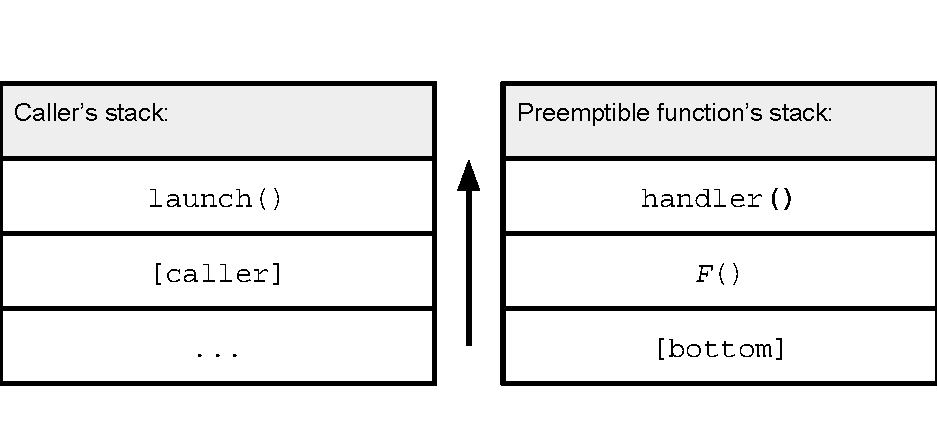
\includegraphics[width=\columnwidth]{figs/twostacks}
\caption{The stacks just after the preemptible function \texttt{\textit{F}()} has been invoked}
\label{fig:twostacks}
\end{figure}

If the function becomes paused, we store its stack in the \texttt{Continuation}
alongside the TCB so neither gets released until the program is done with the
preemptible function.  It is infeasible to relocate a stack in virtual memory while a
preemptible function is paused, so \textit{libinger} currently preallocates large
2-MB stacks to avoid having to resize them (as this should be large enough for any
function that does not stack allocate large locals).  As an implementation shortcut,
it currently allocates the stacks with \texttt{malloc()} and uses a pool
allocator to preallocate and reuse stacks (regardless of whether the preemptible
function ended in cancellation).

Neither of these limitations is fundamental.  If one wanted to avoid preallocating
stacks to reduce startup time and physical memory requirements, one could allocate
stacks with \texttt{mmap()} to avoid faulting the pages.  This technique would also
allow one to make resizeable stacks by requesting even ``bigger'' stacks that would
expand to meet functions' needs (up to some fixed maximum size) using demand paging.
If one needed truly ``boundless'' stack sizes, one could place an unmapped guard page
at the top of each stack; if the stack tried to grow into this space, one would
allocate another stack somewhere else and chain them together with another synthetic
return address.


\section{Signal-based preemption}
\label{sec:libinger:signals}

The defining feature of preemptible functions is that they can be interrupted at any
point.  We implement this external interruption using POSIX interval timers.  The
\texttt{launch()} function calls \texttt{timer\_create()} to request that the kernel
enable fine-grained timer interrupts and periodically signal the process.  When the
signal arrives, control transfers to a handler function in \textit{libinger} that may
decide to pause the preemptible function or let it continue running.  Unfortunately,
the signal is process-directed and gets delivered to an arbitrary thread, not
necessarily the one that is running the preemptible function.

To achieve thread-directed signaling, \texttt{launch()} allocates the current thread
a signal number from a pool.  We use the assigned signal to interrupt this specific
thread.  Once the thread is no longer running a preemptible function, we can release
the signal for use by a different one.  Of course, the signal might still be received
by an unintended thread, so the first thing that our signal handler does is check
whether the arriving signal is assigned to the current thread; if not, it blocks the
signal on that thread.  After as many time periods as the application has threads,
this approach converges to delivering the signal only to its corresponding thread.
Convergence is even faster when reusing a signal from the pool, as it will already
have been blocked by all except one of the threads that existed when it was last used.

A limitation of this design is that the number of kernel threads running preemptible
functions at any given time cannot exceed the number of different signals that the
operating system provides.  Linux currently has 31 standard signals, of which
\textit{libinger} uses up to 16 for preemption.\footnote{This limit could be roughly
tripled by using POSIX real-time signals, although we have not attempted this because
they have slightly different behavior~\cite{signal-manpage}.  Alternatively, glibc on
Linux offers a nonstandard \texttt{SIGEV\_THREAD\_ID} configuration parameter for
directing timer signals at a specific kernel thread; this could be used to remove the
limit (and the pool allocator) entirely~\cite{timercreate-manpage}.}  It currently
assumes that the process will not use any of these signals for other purposes, but
detecting other uses would be as simple as adding forced interposition wrapper
functions for \texttt{signal()} and \texttt{sigaction()}
(Section~\ref{sec:libgotcha:interpose}).

If a signal arrives in the middle of a system call, the system call aborts and
returns an error code.  This is unacceptable because it would mean that moving code
into a preemptible function would introduce spurious error returns from C library and
POSIX functions, which the preemptible function would then have to handle.  When we
install our signal handler, we use \texttt{sigaction()}'s \texttt{SA\_RESTART} flag
to request BSD signal semantics.  This hides the signal arrivals from the preemptible
function by making most standard library functions transparently retry interrupted
system calls.  The \texttt{read()} and \texttt{write()} families of functions change
their behavior in this configuration:\@ blocking calls that have already transferred
some data when the signal arrives will return early, reporting successful completion
and the number of bytes processed.  Programmers using these interfaces should already
defend against the possibility of short counts, so this should not affect correct
programs but might expose existing bugs.  There are also some functions that still
exit with an interruption error code; see Section~\ref{sec:libinger:compatibility}
for further discussion.


\subsection{Interval length and accuracy}
\label{sec:libinger:quantum}

We have described our preemption mechanism, but the question remains of how
frequently the signal handler should check whether the preemptible function has timed
out.  For simplicity, \textit{libinger} currently uses a single fixed scheduling
quantum (timer signal interval) across all preemptible functions.

Before choosing the quantum to use, we were curious how small was achievable with
Linux signals on modern high-precision CPU timers.  We ran an experiment to determine
the effect of a POSIX timer's period on its accuracy.  To measure accuracy, we wrote
a small test program that installs a signal handler and configures a POSIX timer to
trigger it every $T$~\textmu{}s.  Ideally, this handler would always be called
exactly $T$~\textmu{}s after its last invocation; we measured this duration and
recorded the observed deviations from $T$ over 65,535 iterations.  Repeating this
for various values of $T$ showed that the variance is smaller than 0.5~\textmu{}s for
$T \ge$ 3~\textmu{}s, although it exhibits a warmup effect after configuring (or
reconfiguring) the timer.

Of course, at a quantum of 3~\textmu{}s, the CPU will be wasting much of its time on
signal handling.  To assess the overhead of various quanta, we wrote another test
program
that repeatedly computed SHA-512 sums over 64 B of data at a time.  We subjected this
program to \texttt{SIGALRM}s generated by a POSIX timer, varying the quantum and
observing the resulting hashing throughput.  Figure~\ref{fig:shatput} shows that by a
quantum of about 20~\textmu{}s, throughput had reached 90\% of baseline.

\begin{figure}
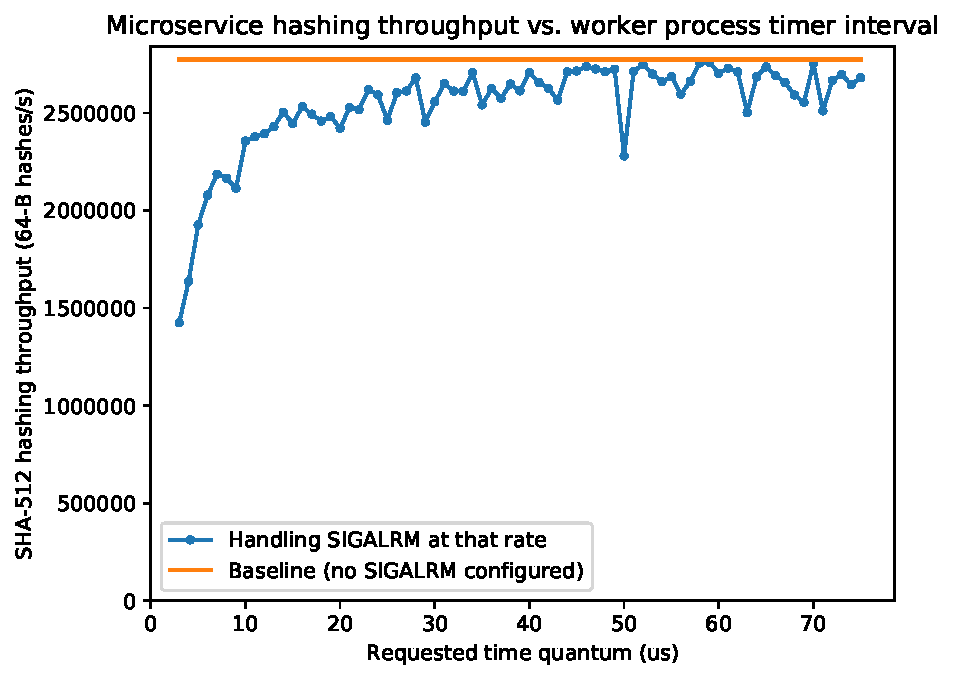
\includegraphics[width=\textwidth]{microservices/figs/2018-02-02-evaluation_quantum-hasher_throughput-throughput}
\caption{Effect of \texttt{SIGALRM} quantum on hashing throughput}
\label{fig:shatput}
\end{figure}

This study shows that it is feasible to support preemption at granularities in the
tens of microseconds, up to two orders of magnitude faster than Linux's default 4-ms
scheduling quantum for processes.  However, it has been our experience that such
small quanta pose a headache during development because they overwhelm debugging
tools such as GDB and Valgrind, causing them to become unresponsive to user input
(even if configured not to deliver the signal to the target program).  To avoid such
problems, \textit{libinger} currently adopts a ``compromise'' quantum of
100~\textmu{}s.

The quantum determines how small a timeout \textit{libinger} can enforce for a
preemptible function.  Note that the quantum represents the duration by which a
preemptible
function might exceed its prescribed timeout:\@ in the worst case, it will exhaust
its time budget infinitesimally long after the handler has interrupted it, and
therefore not be paused until one full quantum later (assuming the timeout is not so
short that the timer is still in its warmup stage).

Competing preemption systems sometimes direct timer signals to a central ``watchdog''
thread that checks whether any tasks are in need of interruption and forwards a
signal to the kernel thread of each that does.  This avoids reducing each preemptible
function's compute throughput at the expense of sacrificing one CPU core.  We instead
opted to use per-thread timer signals for two reasons:  First, assuming most
preemptible functions achieve over 90\% of their baseline throughput as predicted by
our benchmark, it would take more than nine cores constantly running preemptible
functions to break even by committing a watchdog core.  Second, although such a
design may permit preemption quanta in the single-digit microseconds, the gains would
be less in practice because moving the decision to pause to a watchdog core would
increase the worst-case timeout overrun by the latency of propagating the signal
between cores.  Recent measurements place this latency at just under 5,000 cycles on
Linux, which on a 2-GHz processor already represent almost 10\% of the quanta
achievable with marginal throughput cost.  Worse, the sender thread incurs almost
half of this latency~\cite{Kaffes:nsdi2019}, meaning the effect could compound on the
watchdog thread and add to the overrun of other preemptible functions as well.
That said, if an application could not cope with the throughput cost posed by our
approach, would benefit from dropping the preemption quantum by one additional order
of magnitude, or found our signal pool to constrain its scaling, it could revisit
this design decision.

The use of a fixed quantum is not fundamental.  One alternative option is to adjust
the quantum based on the magnitude of the requested timeout, so that the preemptible
function pays a compute overhead proportional to the precision of its time budget.
To be effective, this may require collecting per-machine profiling data on signal
timing characteristics.  A separate enhancement that would benefit longer-running
preemptible functions while still delivering very accurate preemption is to
configure a non-repeating timer to trigger a single signal shortly before the
function was scheduled to time out, then have the handler reconfigure the timer to
repeat with a small quantum for the remainder of the program's run.  The choice of
pre-deadline duration should be informed by the machine's timer signal warmup
behavior.


\section{Pausing a running preemptible function}
\label{sec:libinger:pausing}

We base the decision of whether to pause a running preemptible function on elapsed
wall-clock time, not actual compute time.  One of \texttt{launch()}'s final actions
before invoking the preemptible function is to save a timestamp.  Each time our
signal handler runs, it checks whether the function has exceeded its timeout.  If so,
it pauses it by performing an unstructured jump back to \texttt{launch()} (or
\texttt{resume()}).  Specifically, the location it jumps to is the snapshot captured
earlier, as described in Section~\ref{sec:libinger:contexts}.

While it is possible to call \texttt{setcontext()} from a signal
handler~\cite{getcontext-manpage}, there is an easier way to restore the snapshot.
When installing our signal handler, we set the \texttt{SA\_SIGINFO} flag to request
that each invocation receive more context.  This passes additional arguments to
the handler function, one of which is a POSIX context recording the execution state
just before the signal arrived.  This is also the state that will be restored when
the handler returns, so we implement the jump simply by overwriting it with our saved
snapshot.  Because the context checkpoints the registers including the stack pointer,
returning also switches back to the execution stack of the preemptible function's
caller.

We are only pausing the preemptible function, so the program might later want to
resume it from where it left off.  The preemptible function is already running on its
own stack, and the context passed to the signal handler contains its remaining state.
Before overwriting it, we copy its contents for \texttt{launch()} or
\texttt{resume()} to package into the returned \texttt{Continuation}.
Figure~\ref{fig:twostackscontinuations} shows the state of both stacks and which
frames both continuations point to at the start of the signal handler's execution.
Recall that the snapshot serves as the bridge between the two stacks, and represents
the location that the preemptible function will return to regardless of whether the
handler chooses to pause it.

\begin{figure}
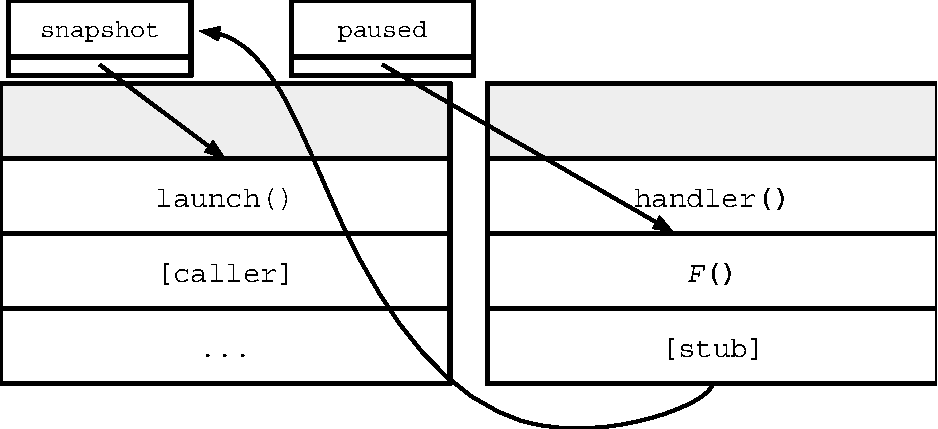
\includegraphics[width=\columnwidth]{figs/twostacks_twocontinuations}
\caption{The stacks and continuations just after \textit{libinger}'s signal handler has been invoked}
\label{fig:twostackscontinuations}
\end{figure}


\subsection{Resuming a paused preemptible function}
\label{sec:libinger:resuming}

\begin{sloppypar}
Should the application resume a paused preemptible function, \texttt{resume()}
repeats many of the transition actions performed by \texttt{launch()}.\footnote{In
fact, there is so much overlap that we implement \texttt{launch()} simply by creating
a \texttt{Continuation}, and then calling \texttt{resume()} if the timeout argument is
nonzero.}  It reuses most resources wholesale from the \texttt{Continuation} object,
but it may need to allocate a new preemption signal (if the application has
transferred the paused preemptible function between kernel threads).  To resume
execution, it must restore the context saved by the signal handler.
\end{sloppypar}

Unfortunately, a restriction in the POSIX specification complicates this unstructured
jump.  The behavior of calling \texttt{setcontext()} on a POSIX context obtained from
a signal handler is unspecified~\cite{getcontext-manpage}, and it is our experience
that glibc's Linux implementation is unreliable in this case.  As a workaround, we
manually raise a signal on the thread and restore the context the same way we
restored the snapshot when pausing, by overwriting the signal handler's context.


\section{Memory isolation and deferred preemption}
\label{sec:libinger:isolation}

There is one final resource that \textit{libinger} allocates for each preemptible
function:\@ a libset (Section~\ref{sec:libsets}).  Here again, it uses a pool
allocator so that each is reused automatically once no longer claimed by any
preemptible function's \texttt{Continuation}.  Recall that a libset represents a copy
of the program's other dynamically-linked modules, and is used to isolate these
modules' nonreentrant state by selectively relinking module entry points against this
copy if they occur within the preemptible function
(Section~\ref{sec:libgotcha:relink}).  Where this approach applies, it happens
transparently to \textit{libinger}.

Recall also that some functions cannot be duplicated in this manner, and instead
require preemption to be deferred until the conclusion of their invocation.  The
\textit{libinger} implementation observes the selective linking rule that the
starting libset is uninterruptible (Section~\ref{sec:libgotcha:unint}).  Before
pausing a preemptible function, the handler checks whether the next libset is equal
to the starting libset.  If so, it blocks the preemption signal and returns without
affecting execution, thereby deferring preemption.  When the running uninterruptible
function returns, \textit{libinger} receives a notification via a control library
callback (Section~\ref{sec:libgotcha:callbacks}) and unblocks the signal again.  To
guard against preemptible functions overrunning their deadlines by calling
uninterruptible functions in a loop, this callback also immediately invokes the
preemption handler, which pauses the function if it has timed out during the
uninterruptible region.

To illustrate the division of responsibility between \textit{libinger} and
\textit{libgotcha}, Figure~\ref{fig:ingerhook} shows an example program that calls a
preemptible function, alongside the resulting control transfers between
modules.\footnote{We depict \textit{libinger} and \textit{libgotcha} as separate
modules for clarity.  However, recall that \textit{libinger} is actually located in
the same module as \textit{libgotcha} because it is an internal control library
(Section~\ref{sec:libgotcha:control}).} \textcircled{1}~The \texttt{main()} function
calls \texttt{launch()} to invoke \texttt{F()} as a preemptible function.
\textcircled{2}~Among \texttt{launch()}'s responsibilities are switching out of the
starting libset and enabling the preemption signal.  At this point, the preemption
handler starts executing periodically and checking whether the preemptible function
is out of execution time.  (If it ever detects a timeout, it will pause the
preemptible function as described in Section~\ref{sec:libinger:pausing}, effectively
skipping to step \textcircled{9}.)  \textcircled{3}~Its setup work complete,
\texttt{launch()} invokes the preemptible function.  \textcircled{4}~This preemptible
function happens to call another function \texttt{callee()} located in a different
module, so \textit{libgotcha} interrupts the call for selective relinking.  There are
two possibilities for what happens next:\@ either \texttt{callee()} is an ordinary
function (in which case \textit{libgotcha} routes the call to the libset's local copy
and we skip to step \textcircled{8} once it returns), or it is an uninterruptible
function.  \textcircled{5}~In the latter case, before transferring control to
\texttt{callee()}, \textit{libgotcha} automatically switches to the starting libset,
deferring preemption.  \textcircled{6}~When \texttt{callee()} returns,
\textit{libgotcha} invokes \textit{libinger}'s callback, which switches back to the
preemptible function's libset and reenables the preemption signal.
\textcircled{7}~The callback raises the preemption signal, and the handler checks
whether the preemptible function has timed out (skipping to step \textcircled{9} if
so).  \textcircled{8}~The function call has completed without timing out, so
\textit{libinger} returns control to the preemptible function.  The preemptible
function happens to return, transferring control back to \texttt{launch()}.
\textcircled{9}~Before returning to \texttt{main()}, \texttt{launch()} switches back
to the starting libset, disabling preemption.

\begin{figure}
	\begin{minipage}{0.25\textwidth}
	\begin{lstlisting}[basicstyle=\footnotesize\ttfamily,tabsize=2,gobble=2]
	int main(void) {

		launch(F, 400, NULL);

	}

	static void F(void *) {

		callee();









		return;




	}
	\end{lstlisting}
	\subcaption{Example program}
	\end{minipage}
%
	\begin{minipage}{0.75\textwidth}
	\includegraphics[width=\textwidth]{figs/calltree_function_launch-crop}
	\subcaption{\vspace{2pt} Corresponding inter-module control transfers (\texttt{callee()} is uninterruptible)}
	\end{minipage}
\caption[Cross-module function calls under \textit{libinger}]{
Cross-module function calls under \textit{libinger}. Solid lines represent function
calls; dashed ones represent returns. Color indicates uninterruptible code (i.e.,
next libset = starting libset).}
\label{fig:ingerhook}
\end{figure}


\subsection{Starting libset exit analysis}

In contrast to the control libraries featured in Chapter~\ref{chap:safety},
\textit{libinger} implements a new abstraction rather than reusing a well-known API
surface.  This allows it to leverage a special \textit{libgotcha} optimization that
was unavailable to the other libraries.  Recall from Section~\ref{sec:libsets} that a
preemptible function, like any isolated task, always runs with its own private next
libset.  Furthermore, the fact that the only way to create a new preemptible function
is by calling the \texttt{launch()} wrapper function means that there is also only
one way for a preemptible function to run with its current libset set to the starting
libset:\@ if it is invoked from the same module that defines it (since otherwise the
caller of the wrapper function would see the function's symbol resolve to a PLOT stub
that would update its current libset from its next one upon invocation).  Isolated
tasks running with their current libset set to the starting one are the only code
regions that can cause an automatic switch \textit{out of} the starting libset (if
they call an interruptible function in any other module).  We know that a preemptible
function with this property can only exist in a module that contains a call to
\texttt{launch()}, so we only have to update the real GOT entries of those starting
libset modules that declare a dependency on \texttt{libinger.so}.  The performance
implications of this insight are significant.  By exempting most of the starting
libset from the runtime overheads of selective relinking, it eliminates all of the
global variable interceptions that would otherwise occur on the critical path of
\texttt{launch()} and \texttt{resume()}.  Furthermore, it eliminates most or all
global variable interceptions that would occur during other uninterruptible function
calls, reducing the risk of significantly exceeding a timeout.  And as we saw in
Section~\ref{sec:gotcha:eval}, each global variable interception incurs several
microseconds of latency.  We call this optimization starting libset exit analysis,
and it should be equally applicable to other
novel task abstractions; a general rule of thumb is that it applies to any control
library whose benefits would not be reaped merely by preloading it.


\section{Calls and returns}
\label{sec:libinger:jumps}

When invoking the preemptible function, there is a possibility that it will throw an
exception.  Most of \textit{libinger} is implemented in Rust, but the process of
switching stacks creates control transfers through C code when calling and returning
from a preemptible function.  It is undefined behavior for Rust panics to cross these
call boundaries~\cite{www-rustlang-ub}, so \textit{libinger} must handle exceptions
specially.  When calling into the preemptible function, \texttt{launch()} stops
exception unwinding by wrapping the call in the standard library's
\texttt{catch\_unwind()} function.  When a preemptible function runs to
``completion,'' \texttt{launch()} and \texttt{resume()} check whether it threw an
exception and call \texttt{resume\_unwind()} if so.  It is possible that applications
seeking to limit functions' execution time might also want to prevent them from
crashing the thread, so one possible revision to the interface would be to provide a
configuration option to skip this rethrow.

The other state that must be transferred between stacks is the preemptible function's
return value, so \texttt{launch()} and \texttt{resume()} store it in an optional type
before switching stacks.  As explained in Section~\ref{sec:libinger:stacks}, each
stack switch returns to the same point regardless of whether the function ran to
completion or timed out and became paused.  To disambiguate these cases,
\texttt{launch()} and \texttt{resume()} check whether they have stored a return
value.  If so, they return it; otherwise, they package a \texttt{Continuation} object
containing the paused function's execution state.


\section{Application compatibility}
\label{sec:libinger:compatibility}

To assess the extent to which \textit{libinger} and \textit{libgotcha} break existing
code, we ran the Gnulib test suite, which exercises hundreds of POSIX and ISO C
library functions.  We ran each test in the suite within a preemptible function by
preloading a library that wrapped \texttt{\_\_libc\_start\_main()} and
\texttt{launch()}ed the program's real \texttt{main()} with an infinite timeout.  On
a glibc 2.29 system, we currently pass approximately 495 of the 519 supported tests
(give or take one or two flaky tests that rely on precise timing behavior affected by
our high-frequency timer signals).

Of the roughly 25 failing tests, most center around functions that we have not
prioritized supporting within preemptible functions:\@ 7 use
\texttt{pthread\_create()} and other thread spawn functions, 6 use \texttt{fork()}
and other process creation functions, and 4 use functions from the \texttt{exec()}
family.  We have not decided what behavior is desirable when a preemptible function
invokes these functions, but the simplest option is to disallow their use by defining
forced interposition replacement functions (Section~\ref{sec:libgotcha:interpose})
that return a failure code when called from within a preemptible function.

Three other recurring issues we encountered were conflicting uses of signals,
replacement of our signal handlers, and interrupted system calls not restarted by
\texttt{SA\_RESTART} (Section~\ref{sec:libinger:signals}).  The former included tests
using historical interfaces such as \texttt{alarm()} that use the same
\texttt{SIGALRM} signal that we allocate for preempting the first preemptible
function.  This is not unexpected because \textit{libinger} does not currently ensure
that its preemption signals are not also used by the program.  The handler
replacement issues mostly involved tests removing our preemption handler by restoring
the default signal disposition.  This would cause the program to crash when the
preemption signal came in, so we worked around it by providing a replacement
\texttt{signal()} wrapper that ignored requests for the \texttt{SIG\_DFL}
disposition.  It is never desirable for a preemptible function to interfere with its
own preemption signal, so a more robust solution would be to add a replacement
wrappers that were aware of its assigned signal and reported failure on all requests
to reconfigure it.  The most frequently recurring functions that did not respect
\texttt{SA\_RESTART} were \texttt{sleep()}, \texttt{usleep()}, and
\texttt{nanosleep()}, which when interrupted return a ``success'' status and the
remaining duration they would have continued to sleep for.  We added replacement
wrapper functions to call them repeatedly using this information.  One function that
returns the \texttt{EINTR} interrupted error code even under \texttt{SA\_RESTART} is
\texttt{select()}, so we added a replacement wrapper that runs it in a loop as long as
this happened.  There are other functions with atypical interruption behavior, and
our system would benefit from systematically adding additional wrappers to hide this
behavior~\cite{signal-manpage}.

A final interesting complication we encountered is that glibc functions that
automatically load supporting dynamic libraries at runtime are not functional by
default in manually-loaded linker namespaces.  For instance, calling the
\texttt{iconv()} family of character set conversion functions causes libc to attempt
to load multiple libraries, each of which performs pairwise conversions between two
specific character sets.  The library attempts to find a minimal sequence of
available pairwise conversions that provides a route between the requested source and
destination character sets; to test whether each candidate pairwise conversion is
supported, it attempts to load a formulaically-named shared library that may or may
not exist.  This means that it is expected that \texttt{dlopen()} may fail, in which
case the dynamic linker will notify \texttt{libc.so} by calling its
\texttt{\_dl\_signal\_exception()} error-handling function.  This function's default
action is to abort the process, so in the case of \texttt{iconv()}, libc updates some
internal state to indicate that this behavior should be suppressed if the call fails.
Unfortunately, the dynamic linker always invokes \texttt{\_dl\_signal\_exception()}
in the main namespace.  In our case, this means that if a preemptible function calls
\texttt{iconv()}, the call is routed to the copy of \texttt{libc.so} in its own
libset, which updates its internal state and then calls into the dynamic linker,
which in turn calls into the starting libset's \texttt{libc.so} that is still
configured to crash on failure.  We work around the problem by defining a replacement
\texttt{\_dl\_signal\_exception()} wrapper that checks the old value of next libset
and reroutes the call to that libset's libc.  The problem and this solution apply to
several other glibc features besides \texttt{iconv()}
(Section~\ref{sec:libgotcha:unintfuns}).

We are confident that with additional engineering effort, it would be possible to
pass the full test suite with the possible exception of the few tests that rely on
precise timing characteristics or incorrectly assume that short blocking file
descriptor I/O operations will not return short counts.


\section{Cancelling a paused preemptible function}
\label{sec:libinger:cancellation}

Should a caller decide not to finish running a timed-out preemptible function, it
must deallocate it.  In Rust, deallocation happens implicitly via the
\texttt{Linger} type's destructor, whereas users of the C interface are responsible
for explicitly calling the \texttt{cancel()} function on the \texttt{linger\_t}
instance.

As discussed in Chapter~\ref{chap:libgotcha}, \textit{libgotcha} returns a
preemptible function's libset to the pool for reuse when that function returns
normally.  However, when a function is cancelled before it finishes, none of the
modules in its libset is safe to reuse in general:\@ a library function might have
been in the middle of executing.  To avoid future problems with the libset, as part
of a cancellation, \textit{libinger} instructs \textit{libgotcha} to reinitialize the
function's libset before returning it to the pool.

Cancellation cleans up \textit{libinger} resources allocated by \texttt{launch()};
however, the current implementation does not automatically release resources already
claimed by the preemptible function itself.  Instead, the preemptible function author
must write a cleanup handler (Section~\ref{sec:safety:acsafe}) and invoke it
immediately before any call to \texttt{cancel()}.  We have, however, created a
prototype
demonstrating the feasibility of automatic cleanup in RAII languages such as Rust,
which we detail in Chapter~\ref{chap:ingerc}.


\section{Evaluation}
\label{sec:libinger:ueval}

Table~\ref{tab:libinger} shows the overhead of \textit{libinger}'s core functions.
Each test uses hundreds of preemptible functions, each with its own stack and
continuation, but sharing an implementation; the goal is to measure invocation time,
so the function body immediately calls \texttt{pause()}.  We show the latencies with
and without the use of dedicated TCBs and TLS areas for each preemptible function
(Section~\ref{sec:libinger:tcbs}).
For comparison, we also measured the cost of calling \texttt{fork()} then
\texttt{exit()}, and of calling \texttt{pthread\_create()} with an empty function,
while the parent
thread waits using \texttt{waitpid()} or \texttt{pthread\_join()}, respectively.

The results show that, as long as preemptible functions are allowed to run
to completion, invoking them incurs a fraction of the latency of spawning a kernel
thread, and an order of magnitude reduction over forking a process.  We collected
these measurements on the same machine using the same software versions as in
Section~\ref{sec:gotcha:eval}.

\begin{table}
	\begin{minipage}{\textwidth}
	\centering
	\begin{tabular}{c | c c}
	Operation & Time with TLSes ($\mu{s}$) & Time without TLSes (\textmu{}s) \\
	\hline
	\texttt{launch()} & $14.4 \pm 0.62$ & $11.8 \pm 0.73$ \\
	\texttt{resume()} & $14.0 \pm 0.74$ & $10.6 \pm 0.38$ \\
	\texttt{cancel()} & $47.5 \pm 5.7$ & $46.9 \pm 2.4$ \\
	\end{tabular}
	\subcaption{Preemptible function operations, with and without per-function TLS areas}
	\end{minipage}

	\begin{minipage}{\textwidth}
	\vspace{12pt}
	\centering
	\begin{tabular}{c | c}
	Operation & Time (\textmu{}s) \\
	\hline
	\texttt{fork()} & $686 \pm 21$ \\
	\texttt{pthread\_create()} & \;\;$68 \pm 18$
	\end{tabular}
	\subcaption{Process and thread spawns without \textit{libinger}}
	\end{minipage}
\caption{Latency of preemptible function interfaces}
\label{tab:libinger}
\end{table}


\subsection{Cancellation response time}
\label{sec:libinger:bombs}

Unlike state of the art approaches, lightweight preemptible functions support
cancellation.

\begin{sloppypar}
\input[functions]{eval_cancel}
\end{sloppypar}

We ran this experiment on an Intel Xeon E5-2683~v4 (Broadwell) server clocked at
2.1~GHz and running Linux~4.12.6, rustc~1.36.0, and glibc~2.29.  As this kernel did
not provide mitigations for the Meltdown or Spectre side-channel attacks, this
configuration is especially favorable for \texttt{fork()} and
\texttt{pthread\_create()} latencies.  We used an older version of \textit{libinger}
predating support for preemptible function--specific TLS and with
\textit{libgotcha}'s global variable interception disabled.  This build relied on our
early, higher-latency approach to libset reinitialization
(Section~\ref{sec:gotchainit}), hence our use of a dedicated reaper thread.
